\subsection{Parton Distribution Functions}
Parton distributions functions (PDFs)  are the densities 
of quarks and gluons carrying a fraction $x$ of the longitudinal hadron momentum.
They  are defined as matrix 
elements in a hadron state of bi-local operators in the light-cone frame, where 
the hadron carries momentum $p$ with plus/minus components
$p^\pm=(p^0\pm p^3)/\sqrt{2}$, and transverse components equal to zero.
%
In the case of unpolarized and polarized quark PDFs, one has
\begin{align}
q(x) & = \frac{1}{4\pi}
\int dy^-e^{-iy^-xp^+}\langle p|\bar{\psi}(0,y^-,\mathbf{0}_\perp)
\gamma^+\mathcal{G}\psi(0,0,\mathbf{0})|p\rangle\,,
\label{eq:LCdefunp}\\
\Delta q(x) & = \frac{1}{4\pi}
\int dy^-e^{-iy^-xp^+}\langle p, s|\bar{\psi}(0,y^-,\mathbf{0}_\perp)
\gamma^+\gamma^5\mathcal{G}\psi(0,0,\mathbf{0})|p, s\rangle\,,
\label{eq:LCdefpol}
\end{align}
where $\psi$ is the quark field and $\mathcal{G}$ is an appropriate gauge link
required to make Eqs.~\eqref{eq:LCdefunp}--\eqref{eq:LCdefpol} gauge invariant.
%
See Refs.~\cite{Collins:1981uw,Curci:1980uw,Baulieu:1979mr,Collins:1989gx} 
for the definition of $\mathcal{G}$ and for
explicit light-cone formul{\ae} of unpolarized an polarized gluon PDFs.
Parton distribution functions are non-perturbative objects that can be determined  from experiment. 

Lattice QCD has also been employed from its early days in order  to calculate PDFs from first principles.  However, the
formulation of lattice QCD in Euclidean space provided a formidable
restriction: the $x$ dependence could not be computed directly, but
only the $x$ moments of the distributions.  Furthermore, the breaking
of rotational symmetry on the lattice in practice restricted such
calculations to only the first few moments. 
The analytic continuation of the matrix elements that define the PDFs to Euclidean space is highly non-trivial due to the fact that these matrix elements are not local in time.
Recently, new ideas have
been proposed that aim to circumvent this
problem~\cite{Ji:2013dva,Ji:2014gla} known as the "Large Momentum Effective Field Theory" (LaMET).
In this approach, one computes a time local version of the matrix element that defines the PDF in Euclidean space given by
%
\begin{equation}\label{eq:qPDF}
h_\alpha(z,p_z) 
= 
\frac{1}{4 p_{\alpha}}\sum_{s=1}^2\left\langle p,s\right\vert \bar{\psi}(z)\gamma_\alpha e^{ig\int_0^z
A_z(z^\prime) dz^\prime} \psi(0) \left\vert p,s\right\rangle,
\end{equation}
%
where $p_\alpha$ is the proton momentum $s$ its spin, and $z$ is the separation of the quark and anti quark fields $\bar\psi$ and $\psi$. A convenient choice is to take the 
proton momentum  and quark, anti-quark separation to be along the $z$ direction (time local) while the Lorentz index $\alpha$ is taken along the time direction $\alpha = 4$~\cite{Xiong:2013bka,Radyushkin:2016hsy,Radyushkin:2017cyf,Orginos:2017kos}. 

With these choices, the quasi-PDF is defined by
\begin{equation}
\widetilde{q}(x,\Lambda,p_z)  
=   \int \frac{dz}{2\pi} e^{-i x z p_z} p_z h_4(z,p_z), 
\end{equation}
where $\Lambda$ is an UV cut-off scale, such as the inverse lattice spacing 
$1/a$. 
In the context of LaMET~\cite{Ji:2013dva,Ji:2014gla}
 this can be related to PDFs using the matching condition
%
\begin{equation} \label{eq:qPDFmatching}
\widetilde{q}(x,\Lambda ,p_z) = 
  \int_{-1}^1 \frac{dy}{\left\vert y\right\vert} 
    Z\left( \frac{x}{y}, \frac{\mu}{p_z}, \frac{\Lambda}{p_z}\right)_{\mu^2 = Q^2} q(y,Q^2) +
  \mathcal{O}\left( \frac{\Lambda_\text{QCD}^2}{p_z^2},\frac{M^2}{p_z^2}\right), 
\end{equation}
where $\mu$ is the renormalization scale,
$Z$ is a matching kernel and $M$ is the nucleon mass.
Here the $\mathcal{O}\left(M^2/p_z^2\right)$ terms are target-mass corrections 
and the $\mathcal{O}\left(\Lambda_\text{QCD}^2/p_z^2\right)$ terms are 
higher-twist effects, both of which are suppressed at large nucleon momentum. 
In the above construction it is assumed that the matrix element  $h_4(z,p_z)$, is renormalized appropriately. 
This can be accomplished using nonperturbative schemes, such as the 
RI/MOM scheme~\cite{Martinelli:1994ty}. This approach has been recently used  for quasi-PDFs  in Refs.~\cite{Alexandrou:2017huk,Chen:2017mzz,Green:2017xeu}.

Alternatively, one can introduce the ratio
\begin{equation}
{\mathcal M}(\nu,z^2) =\frac{h_4(p_z,z)}{ h_4(0,z)}
\label{eq:RatioPseudo}
\end{equation}
where $\nu = p_z z$ is a Lorentz invariant called the Ioffe time~\cite{Ioffe:1969kf,Braun:1994jq}. This ratio is free of UV divergences and requires no renormalization. As shown in~\cite{Radyushkin:2016hsy,Radyushkin:2017cyf} it is related to Ioffe time distributions, which are Fourier transforms of the PDFs through
\begin{equation}
{\mathcal M}(\nu,z^2) =\int_0^1 d\alpha C(\alpha,z^2\mu) {\cal Q}(\alpha x,\mu^2) +{ \cal O}(z^2)
\label{eq:MatchPseudo}
\end{equation}
where  $C(\alpha,z^2\mu^2) $ is a perturbatively calculable function and {\cal Q} is the Ioffe time PDF which relates to the PDF via a Fourier transform 
\begin{equation}
{q}(x,\mu^2)=\int \frac{d\nu}{2\pi} e^{-ix\nu} {\cal Q}(\nu,\mu^2).
\end{equation}


\subsection{Lattice Cross Sections}
Like extracting PDFs from QCD global fits of high energy scattering data, PDFs can also be extracted from analyzing ``data'' generated by lattice-QCD calculation of good {\it lattice cross sections} \cite{Ma:2014jla,Ma:2014jga}. A {\it lattice cross section} is defined as a single-hadron matrix element of a time-ordered, renormalized nonlocal operator ${\cal O}_n(z)$: ${\sigma}_{n}(\nu,z^2,p^2)=\langle p| {T}\{{\cal O}_n({z})\}|p\rangle$ with four-vector, $p$, $z$ and $\nu$ defined above and renormalization scale suppressed. The $p$ and $z$ effectively define the ``collision'' kinematics, and the choice of ${\cal O}_n$ determines the dynamical features of the lattice cross section. A good lattice cross section should have the following three key properties: (1) calculable in lattice-QCD with an Euclidean time, (2) has a well-defined continuum limit as the lattice spacing $a\to 0$, and (3) has the same and factorizable logarithmic collinear (CO) divergences as that of PDFs, which connects the good lattice cross sections to PDFs, just like how high energy hadronic cross sections are related to PDFs in terms of QCD factorization.  

A class of {\it good} lattice cross sections was constructed in terms of a correlation of two {\it renormalizable} currents, ${\cal O}_{j_1j_2}(z)\equiv z^{d_{j_1}+d_{j_2}-2} Z_{j_1} Z_{j_2}\, j_1(z) j_2(0)$, with dimension ($d_j$) and renormalization constant ($Z_j$) of the current $j$.  There could be many choices for the current, such as a vector quark current, $j_q^V(z) = \overline{\psi}_q(z)\gamma\cdot{z}\, {\psi}_{q}(z)$, or a tensor gluonic current, $j_g^{\mu\nu}(z)\propto F^{\mu\rho}(z){F_{\rho}}^\nu(z)$ \cite{Ma:2017pxb}.  Different combinations of the two currents could help enhance the lattice cross sections' flavor dependence.  If $z^2$ is sufficiently small, the lattice cross section constructed from two renormalizable currents could be factorized into PDFs \cite{Ma:2017pxb},
\begin{equation}\label{eq:fac}
{\sigma}_{n}(\nu,z^2,p^2)=\sum_{a}\int_{-1}^1 \frac{dx}{x}\, f_{a}(x,\mu^2) 
K_{{n}}^{a}(x\nu,z^2,x^2p^2,\mu^2) +O(z^2\Lambda_{\rm QCD}^2)\, ,
\end{equation}
where $\mu$ is the factorization scale, $K_n^{a}$ are perturbatively calculable hard coefficients, and $f_{a}$ is PDF of flavor $a=q,g$ with anti-quark PDFs expressed by quark PDFs using the relation $f_{\bar{a}}(x,\mu^2)=-f_{{a}}(-x,\mu^2)$.  PDFs could be extracted from global fits of lattice-QCD generated data for various lattice cross sections $\sigma_{n}(\nu,z^2,p^2)$ with corresponding perturbatively calculated coefficients $K_n^{a}$ in Eq.~(\ref{eq:fac}).

The quasi-PDFs and pseudo-PDFs introduced above could be derived by choosing 
\begin{equation}
{\cal O}_{q}(z)=Z_q(z^2)\overline{\psi}_q(z)\gamma\cdot {z}\, \Phi(z,0){\psi}_q(0)\,.
\end{equation}
 with the renormalization constant $Z_q(z^2)$ and the path ordered gauge link $\Phi(z,0)={\cal P}e^{-ig\int_0^{1} z\cdot A(\lambda z)\,d\lambda}$ \cite{Ma:2017pxb}.  With $K^{q(0)}_{q}(x \nu,z^2,0,\mu)= 2 x \nu  e^{i x \nu}$, one finds,
\begin{equation}\label{eq:lcsQuasi}
\int \frac{d \nu}{\nu}\, \frac{e^{-i x \nu}}{4\pi} \sigma_{q}(\nu,z^2,p^2)\approx f_{q}(x,\mu)\, ,
\end{equation}
modulo $O(\alpha_s)$ and higher twist corrections.  By choosing $z_0=0$ and both $\vec{p}$ and $\vec{z}$ along the ``3"-direction, one finds that $\nu=-z_3\, p_3$ and the left hand side of Eq.~(\ref{eq:lcsQuasi}) is the quasi-quark distribution introduced in Ref.~\cite{Ji:2013dva} if the integral is performed by fixing $p_3$, while it is effectively the pseudo-quark distribution used in Ref.~\cite{Orginos:2017kos} if the integral is performed by fixing $z_3$. That is, these two approaches for extracting PDFs are equivalent if matching coefficients are calculated at the lowest order in $\alpha_s$ neglecting all power corrections, but different if contributions from either higher order in $\alpha_s$ or higher powers in $z^2$ need to be considered.
 %That is, these two approaches for extracting PDFs are equivalent if matching coefficients are calculated to the lowest order in $\alpha_s$, but different if higher order contributions need to be considered. 
Furthermore, Eq.~(\ref{eq:lcsQuasi}) indicates that the quasi-PDFs and pseudo-PDFs are two special cases of good lattice cross sections. 




\subsection{Generalized Parton Distribution Functions}





\subsection{Gluon observables}

\subsubsection{Motivation and Achievement}


While gluons and the QCD interactions they embody play an essential role in the binding of hadrons, gluon contributions to hadron structure observables are far less well known than their quark analogues. A primary mission of the proposed Electron-Ion Collider~\cite{Accardi:2012qut,Kalantarians:2014eda}, which is the highest priority for new construction in the NSAC nuclear physics long-range plan~\cite{Geesaman:2015fha}, is to image the gluon structure of hadrons and nuclei. This program will access the three-dimensional gluon structure of the nucleon and allow first measurements of gluon GPDs and TMDs, complimenting significant efforts at RHIC to measure the gluon contribution to the nucleon spin, and potential experiments to study gluon distributions at JLab~\cite{Maxwell:2018gci,Hattawy:2017woc,Dobbs:2017vjw} and at the LHC~\cite{Baltz:2007kq}. 
%
In this light, LQCD calculations of gluon structure quantities have taken on renewed importance. There has been significant progress on this front over the last five years~\cite{Alexandrou:2017oeh,Yang:2016plb,Detmold:2016gpy,Detmold:2017oqb,Winter:2017bfs}, expanding and building on pioneering studies of the unpolarised gluon structure of the pion and nucleon~\cite{Meyer:2007tm,Horsley:2012pz,Alexandrou:2013tfa} over the last decade. 

In particular, LQCD calculations have provided new insight into the proton spin crisis---the realization that quarks carry only a relatively small fraction of the proton spin---by way of complete and fully-controlled determinations of the key and poorly-known gluon contributions to the nucleon spin~\cite{Alexandrou:2017oeh,Yang:2016plb}. 
These results include a significantly improved constraint on the total gluon helicity~\cite{Yang:2016plb} compared to global analyses of polarized parton distributions~\cite{deFlorian:2014yva}.
Complementing these works, new understanding of the continuum of decompositions of the nucleon spin in the LQCD framework has been achieved~\cite{Engelhardt:2017miy}, and studies of the non-perturbative~\cite{paper by Yibo et al to appear next week} and perturbative renormalization~\cite{Alexandrou:2017oeh} of gluon operators have begun.
%
In another impressive success, the gluon contribution to the nucleon's momentum has been resolved at 10\% precision, with the momentum sum rule (including separate determinations of the quark and gluon connected and disconnected contributions) found to be satisfied at quark masses corresponding to the the physical value of the pion mass~\cite{Alexandrou:2017oeh}. Extensions of this work will rival the precision of phenomenological parton distribution fits (e.g., CT14NNLO~\cite{Dulat:2015mca}) in the next few years.
%
First calculations of some of the moments of the gluon GPDs~\cite{Diehl:2003ny} that describe the distribution of gluons in hadrons both in the transverse plane and in the longitudinal direction~\cite{Detmold:2016gpy,Detmold:2017oqb} have also been performed, providing first insight into details of the three-dimensional gluon structure of hadrons, albeit without fully-controlled uncertainties. 
Moreover, aspects of the gluon structure of nuclei have been studied for the first time, {\color{red} as described in Section~\ref{}}.

The following subsection outlines the prospects for LQCD calculations of the gluon structure of hadrons on a 5-year timescale. It is expected that in this time many key gluon structure quantities will be calculated at 2-5\% precision with fully-controlled uncertainties, and others will be accessed for the first time, providing new insight into hadron structure and serving as QCD predictions and benchmarks for the EIC and other experimental programs.

%\begin{figure}[t]
%	\includegraphics[width=0.45\textwidth]{vbars-xudsg2.pdf}
%	\caption{\label{fig:momfrac}Figure taken from Ref.~\cite{Alexandrou:2017oeh}, which includes a physical-mass calculation of the fraction of momentum carried by gluons in the nucleon (green vertical bar labeled `g').}
%\end{figure}



\subsubsection{Future opportunities gluons}

Exascale computing resources and concurrent algorithm development {\color{red} (see Section~\ref{})} will facilitate LQCD calculations of static gluon structure quantities with fully controlled uncertainties. Given recent advances that significantly lower the cost of gauge field generation {\color{red} (see Section~\ref{})}, calculations on multiple large lattice volumes (e.g., $L^3\times T=72^3 \times 192$ and larger) will achieve significant advantages through volume averaging which acts to reduce the gauge noise that is a statistical challenge for calculations of gluon observables. Nevertheless, these studies face significant analysis costs and achieving controlled calculations of non-static quantities including the distributions that encode the three-dimensional gluon structure of the nucleon, especially at large momenta (as required to extract the $x$-dependence of PDFs, GPDs and TMDs) and in the approach to the continuum limit (where gluon field fluctuations grow), will require continued development of algorithms and new analysis approaches.\\


{\it Static properties of the nucleon}

In the near term, precise calculations of moments of gluon distributions encoding the contribution of gluons to the mass, momentum, and spin of the nucleon and of other hadrons will be refined. In particular, one can expect calculations at quark masses corresponding to the physical pion mass with fully-controlled uncertainties at the level of 2-5\% precision. 
To achieve this level of systematic control, it is necessary to precisely determine the required renormalizations, including mixing between the gluon observables and the flavor-singlet quark disconnected terms. This carries significant computational cost in its own right.\\
 

{\it Form factors and radii}

The gluon radius of the nucleon is a quantity as fundamental as the charge radius, but it is not known quantitatively or qualitatively, from experiment or theory, how the charge and gluon radii compare. 
Defined by the slope of the spin-averaged gravitational form factor at zero momentum transfer, the gluon density radius is related via the operator product expansion to matrix elements of the gluon part of the energy-momentum tensor.
This, and more generally the $Q^2$-dependence of the generalized gluon form factors that describe the moments of the gluon GPDs, can be calculated using LQCD for both hadrons and light nuclei~\cite{Detmold:2017oqb,Winter:2017bfs}.
On a few-year timescale, fully-controlled calculations of gluon generalized form factors for the nucleon, for low moments and to a scale of several GeV$^2$, can be expected.
From experiment, comparison of nuclear quark and gluon radii will likely be possible through measurements of the parton densities in ${}^4$He at the JLab 12 GeV program~\cite{Hattawy:2017woc}, or from direct measurements of nuclear and nucleon gluon densities using heavy quark production at the planned EIC~\cite{Chudakov:2016otl}. \\


{\it PDFs and TMDs}

In the longer term, coinciding with the era of exascale computing, one can expect that the $x$-dependence of gluon PDFs and TMDs will be determined from LQCD. Defined on the lightcone, these quantities can not be calculated directly on a Euclidean lattice but can be accessed via rotations to `quasi' or `pseudo' PDFs, extrapolated back to the physical quantity in the large-momentum limit. For the quark PDFs and TMDs these approaches have shown great promise and early success~\cite{Lin:2014zya,Alexandrou:2015rja} ({see also \color{red} Section~\ref{)}}). Ultimately, extending these calculations to include gluon distributions will allow a complete decomposition of the three-dimensional quark and gluon structure of the nucleon.\\



\subsubsection{TMDs}

{\it TMDs: Motivation and Achievements}
Transverse momentum-dependent parton distributions (TMDs) \cite{Boer:2011fh}
constitute one of the pillars on which the three-dimensional tomography of
hadrons rests. Together with the three-dimensional spatial information
derived from generalized parton distributions (GPDs), they permit a
comprehensive reconstruction of hadron substructure and thus
have a bearing on seminal topics in hadron physics, such as
orbital angular momentum contributions to nucleon spin, or
spin-orbit correlations in hadrons. Through the selection of
particular parton spin and transverse momentum components, a
variety of effects can be probed, including naively time-reversal odd
(T-odd) quantities such as the Sivers and Boer-Mulders functions;
these only exist by virtue of initial or final state interactions
in corresponding physical processes, introducing a preferred chronology
in the description of the process.
For example, in semi-inclusive
deep inelastic scattering (SIDIS), the operative element is final-state
interactions between the struck quark and the hadron remnant; on
the other hand, in the Drell-Yan (DY) process, initial state interactions
before the lepton pair production enable T-odd effects.

In view of the fundamental importance of TMDs and the rich spectrum of
effects that can be probed, TMDs have been, and continue to be the
target of a variety of experimental efforts. Deep-inelastic scattering
experiments performed by COMPASS \cite{Alekseev:2008aa,Adolph:2014fjw},
HERMES \cite{Airapetian:2009ae,Airapetian:2013bim} and Jefferson Lab
\cite{Qian:2011py,Avakian:2010ae} have yielded TMD data including evidence
for the T-odd Sivers effect. Complementary Drell-Yan experiments at
COMPASS \cite{Gautheron:2010wva} and Fermilab \cite{Brown:2014sea} are
envisaged, which could, in particular, test the sign change between
the SIDIS and DY processes. Related transverse single-spin
asymmetries have been measured at RHIC in polarized proton-proton
collisions \cite{Adare:2013ekj,Adamczyk:2012xd}. Further experimental
efforts at RHIC are projected to provide insight into strong QCD evolution
effects expected for the Sivers TMD \cite{Echevarria:2014vda}.
TMDs furthermore constitute a central focus of the proposed Electron-Ion
Collider facility \cite{Accardi:2012qut}.

\begin{figure}[h!]
\centering
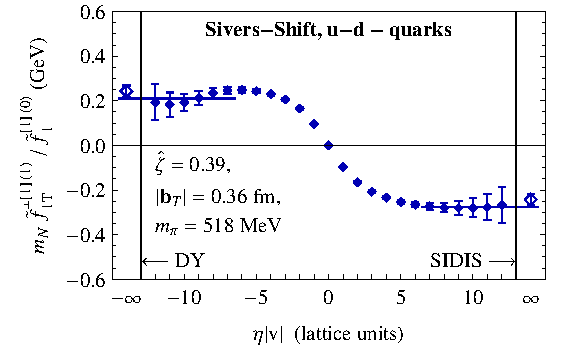
\includegraphics[width=0.474\columnwidth]{pdfs/figures/m020_run38_UminusD_Sivers_lsqr-9_zetasqrlat4}\hspace{1cm}
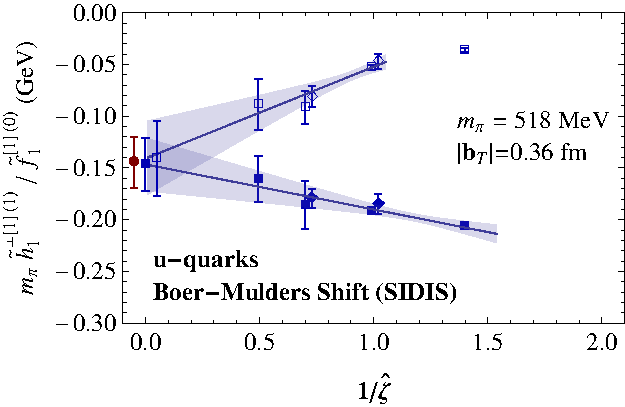
\includegraphics[width=0.45\columnwidth]{pdfs/figures/new_bm_u_sidis_b0p36_vszetahat_extrap_pow1}
\caption{Left: Proton Sivers shift as a function of staple length for fixed
staple width $b_T $ and rapidity (Collins-Soper) parameter $\hat{\zeta } $;
$\eta \rightarrow \infty $ defines the SIDIS limit \cite{Musch:2011er}.
Right: Extrapolation of the SIDIS limit data for the pion Boer-Mulders
shift to the physical limit of large $\hat{\zeta } $
at fixed $b_T $ \cite{Engelhardt:2015xja}. Open symbols represent a partial
contribution that dominates at large $\hat{\zeta } $, providing further
insight into the approach to the asymptotic regime.}
\label{fig_sidis}
\end{figure}

To complement and support these efforts, a sustained
project to calculate TMD observables within lattice QCD was initiated
and developed in \cite{Hagler:2009mb,Musch:2010ka,Musch:2011er,Engelhardt:2015xja,Yoon:2017qzo,Engelhardt:2017miy}.
TMDs are formally defined through matrix elements of a bilocal quark
operator in which the quark fields are connected through a gauge link
along a staple-shaped path. Building on the preliminary investigations
\cite{Hagler:2009mb,Musch:2010ka}, the first full calculation of TMD
observables using staple-shaped gauge links was performed in
\cite{Musch:2011er}, obtaining results on the Sivers and Boer-Mulders
shifts, a worm-gear shift, and the generalized transversity.
Fig.~\ref{fig_sidis} (left) displays a typical result for the Sivers
shift, exhibiting its T-odd character and the SIDIS and DY limits
achieved for asymptotic staple length.

Such lattice TMD calculations face several challenges. One is achieving
the physical limit of large rapidity difference between between struck
quark and hadron remnant in a deep inelastic scattering process, which
is encoded in the space-time direction of the staple link. An investigation
of the Boer-Mulders shift in a pion dedicated to elucidating this limit
was reported in \cite{Engelhardt:2015xja}. A result from this study is
shown in Fig.~\ref{fig_sidis} (right), demonstrating access to the large
rapidity regime. Another challenge is understanding renormalization,
operator mixing and scaling. Observables such as the Sivers shift are
constructed as ratios in which certain renormalization factors cancel
in continuum QCD; to test whether this pattern persists in the lattice
formulation, a comparison between TMD calculations on clover and domain
wall fermion ensembles at approximately the same pion mass was performed
and reported in \cite{Yoon:2017qzo}. Fig.~\ref{tmd_comp} (left) displays
consistent results for the Sivers shift, corroborating the cancellation
of renormalization factors expected from continuum QCD. On the other hand,
in the case of the worm-gear shift, operator mixing is predicted for
clover fermions \cite{Constantinou:2017sej}, which destroys the simple
cancellation in ratios; evidence for this was also seen in the data
collected in \cite{Yoon:2017qzo}. A third challenge for lattice TMD
calculations is progress towards the physical pion mass. After a
preliminary study \cite{Engelhardt:2015czw}
at a pion mass of $m_{\pi } = 170\, \mbox{MeV} $,
which still suffered from substantial statistical uncertainties,
a current 150 Mch INCITE allocation is dedicated, with USQCD endorsement,
to the large-scale production of lattice TMD data at the physical pion mass.
This program includes the use of boosted nucleon sources to access the
large rapidity regime, as well as excited state control through
calculation for a range of source-sink separations.

\begin{figure}[h!]
\centering
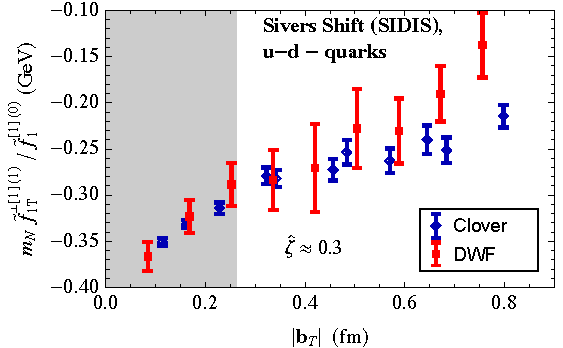
\includegraphics[width=0.462\columnwidth]{pdfs/figures/UminusD_SiversRat_zetahat-0p35_bdepend_comb}\hspace{1cm}
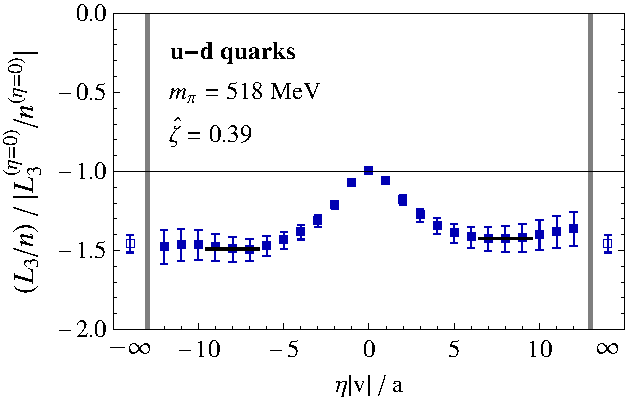
\includegraphics[width=0.45\columnwidth]{pdfs/figures/etaplot_umd_zeta39}
\caption{Left: Comparison between SIDIS limit data for the proton Sivers
shift obtained for two distinct lattice discretizations, as a function of
staple width $b_T $ at fixed rapidity parameter $\hat{\zeta } $
\cite{Yoon:2017qzo}. Right: Longitudinal quark orbital angular momentum
(OAM) in the proton $L_3 $ as a function of staple length at fixed
$\hat{\zeta } $ \cite{Engelhardt:2017miy}. The limit $\eta =0$ yields Ji
OAM, $\eta \rightarrow \pm \infty $ Jaffe-Manohar OAM. The ratio of $L_3 $
to the number of valence quarks $n$ is evaluated to cancel multiplicative
renormalizations. Data are shown in units of the absolute value of Ji OAM.}
\label{tmd_comp}
\end{figure}


In addition to the aforementioned calculations, which concentrated on
transverse momentum dependence while integrating over longitudinal
momentum fraction $x$, exploratory data have also been gathered on the
$x$-dependence of the Sivers shift, achieved by adding a
longitudinal separation in the bilocal quark operator defining TMDs.
These data are awaiting analysis. Furthermore, the generalization
of TMDs to non-zero momentum transfer (GTMDs) was explored in
\cite{Engelhardt:2017miy}, with a specific focus on the direct
calculation of quark orbital angular momentum (OAM) in the proton.
Considering non-zero momentum transfer supplements the transverse
momentum information with transverse position information, thus
yielding direct information on OAM (as opposed to indirect access
as $L=J-S$ via Ji's sum rule). Moreover, this approach allows one
to not only calculate Ji OAM, but also Jaffe-Manohar OAM.
Fig.~\ref{tmd_comp} (right) displays a gauge-invariant, quasi-continuous
interpolation between these two OAM definitions from \cite{Engelhardt:2017miy}.
Currently, this first calculation is being improved upon by employing a
direct derivative method to treat the derivative with respect to
momentum transfer needed to extract OAM.

{\it TMDs: Future program and resource requirements}
The investigations described above provide the necessary foundation for
the controlled, precise prediction of selected TMD observables from
lattice QCD. The chief systematic challenges have been explored,
and a tentative roadmap of incremental refinement of the calculations can
be projected. As already implemented within the current INCITE project,
the use of boosted nucleon sources will allow access to the large
rapidity regime. Discretization effects will need to be quantified
as momenta are increased. This, as well as a quantitative treatment
of the renormalization and QCD evolution of lattice TMD observables,
building on the initial study \cite{Yoon:2017qzo}, will necessitate a
sequence of calculations with decreasing lattice spacings.

In assessing the required resources, it should be noted that lattice
TMD calculations are dominated by the cost of the large number of
contractions, as opposed to the cost of the inversions needed to
obtain propagators. TMD calculations are unique in this respect;
the large number of contractions results from the multitude of
staple-shaped gauge link geometries that must be surveyed in order
to perform the necessary extrapolations to long staple length as
well as large rapidity difference between struck quark and hadron
remnant in a deep-inelastic scattering process. This characteristic
allows for a fairly simple estimate of the computing costs. Keeping
physical parameters constant, the costs scale as the inverse 4th power
of the lattice spacing. Thus, to perform a calculation at half the
currently employed lattice spacing requires 16 times the resources.
Combining this with the volume of the current INCITE allocation of
150 Mch, a lattice TMD project at the physical pion mass and lattice
spacing around 0.05 fm will require resources of the order of
2 Gch.

In connection with the renormalization of lattice TMD observables,
also the operator mixing induced in selected quantities by the clover
fermion discretization needs to be taken into account. Whereas this
mixing can be avoided by using chirally symmetric domain wall fermions,
we envisage utilizing also the large set of clover ensembles generated
by the W\&M/JLab collaboration for TMD studies. A scheme along the lines
put forward, e.g., in \cite{Green:2017xeu} will serve to incorporate mixing
effects in clover calculations.

A further aspect that remains to addressed is the flavor separation
of TMD observables and sea quark effects, as targeted, e.g., by the Fermilab
E-906/SeaQuest experiment. This calls for the evaluation of disconnected
diagram contributions, which hitherto have not been studied in lattice TMD
investigations. An efficient calculation of these diagrams will be possible
employing hierarchical probing methods \cite{Stathopoulos:2013aci}.
Based on our experience
in the context of form factor calculations \cite{Green:2015wqa}, these methods
can yield disconnected contributions at about twice the cost of the connected
contributions. Thus, a fully flavor-separated calculation including
quark loops requires altogether about three times the resources compared
to a calculation of the connected contributions only. This factor has to
be compounded with the estimates made above. It should moreover be
noted that this does not yet take into account the mixing of gluonic
operators with flavor singlet quark operators. Incorporating this mixing
is an additional component which is yet to be explored in the context
of lattice TMD calculations.

Complementary to these improvements of the systematics of lattice TMD
calculations, also the incorporation of further physics objectives is
envisaged. To date, our calculations have focused on transverse nucleon
polarization, with which one can probe the particularly interesting
Sivers and Boer-Mulders effects. Nonetheless, also the TMDs associated
with longitudinal nucleon polarization are of interest and include a
second worm-gear function in addition to the one probed with transverse
polarization. TMD calculations with longitudinal polarization are
straightforward to implement in the existing scheme. Furthermore, the
extension of lattice calculations to include the $x$-dependence of TMDs,
already explored for the case of the Sivers shift as noted above, must be
continued to encompass a variety of TMD observables.

In addition, the study of GTMDs, i.e., TMDs in the presence of a
momentum transfer, must be extended beyond the specific case of quark
orbital angular momentum already highlighted further above
\cite{Engelhardt:2017miy}. For example, spin-orbit correlations of quarks
in the proton can be quantified through the GTMD $G_{11} $ in the
classification scheme of \cite{Meissner:2009ww}.
Also complementary ways of accessing quark orbital
momentum, e.g., through the twist-3 GTMDs $F_{27} $, $F_{28} $, related
to the GPD $\widetilde{E}_{2T} $, will be explored.



{\it Hybrid mesons}

There is considerable experimental evidence for mesonic states that do not fit into a constituent quark model picture~\cite{Patrignani:2016xqp}; it is theorised that bound gluons (glueballs), or $q\overline{q}$-pairs bound with excited gluons (hybrids), may account for these observations. 
As highlighted in the 2015 NSAC long-range plan~\cite{Geesaman:2015fha}, LQCD plays an essential role in guiding experiments designed to search for exotic states, including the flagship GlueX experimental program at JLab~\cite{Dobbs:2017vjw}. In addition to specroscopic studies of the resonances in question {\color{red}(see Section~\ref{})}, LQCD studies of their three-dimensional gluon structure described by the gluon GPDs and TMDs may provide insight from QCD into details of the nature of exotic states. These calculations are extremely demanding computationally and will also require continued theoretical development.
